%Aufbau eines Dokumentes
%Jedes LaTeX-Dokument besteht aus einer Präambel und einem Dokumentenkörper. Im folgenden werden beide an jeweiliger Stelle beschrieben.
%1. Präambel
%In der Präambel wird die Dokumentenklasse definiert und weitere wichtige Bestimmungen, die global (also für das ganze Dokument) gelten werden. Dazu gehören beispielsweise Einstellungen für die Sprache im Dokument, für die Schriftart, für die Ränder und alles, was eben zu den Grundlagen, die jedes Dokument erfüllt dazugehört. LaTeX bietet einem viele Optionen, die es möglich machen, das Dokument frei zu gestalten. Die meisten werden in Form von sogenannten Usepackages eingebunden. Alle folgenden Usepackages werden von mir kommentiert. Mit der Zeit werden weitere dazukommen. Das Schöne an Usepackages ist, dass sie von jedem erstellt werden können und damit jeder an LaTeX mitschreiben kann.
\documentclass{article}
%Die Dokumentenklasse article ist wahrscheinlich die am häufigsten verwendete Klasse und dient dazu kurze und mittellange Dokumente zu erstellen. Es sollten ein paar Dinge auffallen.
%1. Jeder Befehl in LaTeX startet mit einem \ (Auf deutschen Tastaturen AltGr + ß) Das, was hinter dem \ steht wird solange zum Befehl gezählt, bis erstmals ein Leerzeichen oder eine Zahl oder ein Sonderzeichen kommt.
%2. Typischerweise stehen die Klammern hinter dem Befehl für die Dokumentenklasse und die Usepackages für zwei Dinge. In die geschweiften {} Klammern kommt der Name der Klasse/des Pakets. In die eckigen [] Klammern kommen mögliche Spezifikationen. Hier ist der Name der Klasse article. Es gibt auch beamer (für Präsentationen) und viele weitere Klassen, die allerdings seltener als diese zwei verwendet werden (beispielsweise die Klasse book, die sich für längere Dokumente unter Umständen besser als die Klasse article eignet).
\usepackage[ngerman]{babel}
%Das Usepackage babel erlaubt es voreingestellte Konfigurationen für bestimmte Sprachen zu verwenden. Das umfasst beispielsweise Dinge wie, dass die Überschrift vom Inhaltsverzeichnis automatisch Inhaltsverzeichnis und nicht Table of contents heißt, oder dass unter Abbildungen nicht figure sondern Abbildung steht. Solche Dinge könnte man alle auch selbst einstellen, jedoch erleichtern usepackages das enorm. Zudem sollte man spätestens hier bemerken, dass man, wenn man sich einmal eine Vorlage aus usepackages ect. zusammengebastelt hat, man diese Vorlage immer wieder verwenden kann und die eigenen Dokumente dann automatisch einen einheitlichen Stil bekommen.
\usepackage[utf8]{inputenc}
\usepackage[T1]{fontenc}
%Die Usepackages inputenc und fontenc dienen dazu, den Zeichensatz, der verwendet werden soll anzupassen. Wir gehen da hier nicht tiefer drauf ein, da es ein einführender Kurs sein soll. Weitere Informationen findet man massenweise im Internet, es reicht sowas wie "LaTeX inputenc" zu googlen.
\usepackage{hyphenat}
\hyphenation{Mathe-matik wieder-gewinnen}
%Diese beiden Befehle (also Paket + Befehl \hyphenation) dienen dazu festzulegen, wo LaTeX bei einem Wort, wenn es auf zwei Zeilen gebrochen werden soll, einen Umbruch setzen soll.
%Bibliographie
\usepackage{biblatex}
\addbibresource{literature.bib}

\usepackage{amsmath}
\usepackage{amsfonts}
\usepackage{amssymb}
\usepackage{amsthm}
%Diese vier Pakete binden den gesamten Mathesatz der American Mathematical Society ein und sollten standardmäßig eingebunden werden. Auch hier verweise ich an dieser Stelle alle Neugierigen für weitere Informationen erstmal an das Internet.
\usepackage{hyperref}
\hypersetup{
colorlinks=true,
linkcolor=red
}

\usepackage{graphicx}
\graphicspath{ {./Bilder/} }
\usepackage{float}
\usepackage{subcaption}

\usepackage{geometry}
\geometry{left=2cm, right=2cm, top=2cm, bottom=3cm,a4paper}
\usepackage[normalem]{ulem}
\useunder{\uline}{\ul}{}
\newcommand{\rund}[1]{\left(#1\right)}
\newcommand{\eck}[1]{\left[#1\right]}
\newcommand{\intd}[1]{\text{d}#1}
\title{Mein erstes \LaTeX-Dokument}
\author{Amin Thainat}
\date{\today}
%Hier kann nun ein Titel, ein Autor und ein Datum festgelegt werden, wenn man möchte, dass LaTeX die auf eine standardmäßige Art und Weise einbindet. Später kann man sowas auch für die eigenen Bedürfnisse anpassen. Hier definiert man aber, wie es für alles in der Präambel so ist, diese Parameter (Titel, Autor, Datum) global. \today ist ein Befehl, der einfach das aktuelle Datum ausgibt. Je nachdem, welche Dokumentensprache mit dem Paket babel festgelegt wurde, sieht das Datumsformat in der Ausgabe entsprechend anders aus.

%Man sollte sich zu den Paket und der Dokumentklasse hier noch merken, dass all diese Pakete in ihrer Art (für ein deutschsprachiges Dokument) zum Standard gehören. Sie ändern an der Konfiguration des Dokumentes (wie beispielsweise den Rändern) noch nichts.

%2. Dokumentenkörper
%Im Dokumentenkörper steht nun der eigentliche Text, der auch später im Dokument erscheinen soll. Nach und nach werden wir lernen, wie man die wichtigsten Sachen in LaTeX umsetzen kann.
%Der Dokumentenkörper ist in LaTeX eine sogenannte Umgebung. Umgebungen werden immer mit \begin{Umgebungsname} geöffnet und mit \end{Umgebungsname} geschlossen. Alles, was in einem LaTeX-Dokument nach \end{document} steht, ist für das Dokument irrelevant.
\begin{document}
	\maketitle
	%Der Befehl maketitle fügt das eingestellten Titel+Autor+Datum in einer meist von der Dokumentenklasse abhängigen Weise automatisch an der Stelle, wo der Befehl steht, hinzu.
	\tableofcontents
	%Der Befehl \tableofcontents fügt an der Stelle, wo er steht, automatisch ein Inhaltsverzeichnis hinzu. Das ist ein sehr praktisches Werkzeug, das LaTeX bietet, denn das Inhaltsverzeichnis wird immer automatisch aktualisiert. (Manchmal muss man das Dokument zweimal kompilieren, damit das Inhaltsverzeichnis aktualisiert ist. Kompilieren tut man in TeXStudio indem man auf den grünen Doppelpfeil in der Leiste oben klickt.)
\section{Mein erstes Kapitel}
%Man kann in LaTeX verschiedene Ebenen von Kapiteln erstellen. Typischerweise ist die höchste Ebene, die man einem Artikel verwendet eine Section. Sections und auch subsections ect. sind KEINE Umgebungen, sie werden also nicht mit \begin{} und \end{} aufgerufen. Eine section ist einfach da zuende, wo eine neue startet.
Dieses Kapitel wurde in unserem ersten Lernraum erstellt. 
%Normaler Text wird auch einfach normal geschrieben. :)
Später diskutieren wir das eingeschobene Unterkapitel, siehe Kapitel \ref{subsec:eingeschobenesUnterkapitel}.
$1+1=2$, $\frac{a}{b}$.
\begin{equation}
a^2+b^2=c^2
\end{equation}
%Formeln, die im Text stehen sollen, begrenzt man durch $-Zeichen. Alles, was zwischen zwei $-Zeichen steht, ist im sogenannten Mathemodus. Alles, was mit Formeln ect. zu tun hat, sollte im Mathemodus stehen. $\frac{}{}$ ist ein Bruch, wobei in den ersten geschweiften Klammern der Inhalt des Zählers und in den zweiten geschweiften Klammern der Inhalt des Nenners steht.
\begin{equation}
	U_{\nu}^{o}(\nu,T)\intd{\nu}
	=
	\frac{8\pi h\nu^3}{c^3}
	\frac{1}{e^{\frac{h\nu}{kT}}-1}\intd{\nu}\label{eq:Strahlungsgesetz}
\end{equation}
%Man kann auch ganze Zeilen für den Mathemodus reservieren, das lohnt sich vor allem dann, wenn man längere Ausdrücke oder Gleichungen tippen möchte. Die entsprechende Umgebung heißt equation. (Wie immer: Da equation eine Umgebung ist, wird sie mit \begin{equation} begonnen und mit \end{equation} beendet.)
%Diese Gleichung (der Inhalt ist jetzt irrelevant) enthält einige Zeichen, die ich jetzt erkläre. \nu und \pi sind die kleinen griechischen Buchstaben nü und pi. Alle griechischen Buchstaben lassen sich so tippen, die jeweilige große Version erhält man, indem man den ersten Buchstaben des Befehls groß schreibt, also beispielsweise \Pi. Mit dem Zirkumflex, ^ , stellt man Ausdrücke hoch. Möchte man nur ein einziges Symbol hochstellen, kann man das direkt hinter das ^-Zeichen schreiben, möchte man mehrere Ausdrücke hochstellen, so schreibt man ^{...}, wobei ... alles ist, was hochgestellt sein soll. Dasselbe gilt für _ bei der Tiefstellung. Das Schöne ist, dass man all diese Dinge im Prinzip nach Belieben kombinieren kann, also beispielsweise, wie auch hier in der Formel, dass man im Nenner eines Bruches einen Exponenten hat, in dem wieder ein Bruch steht. Probiert aus, damit ein wenig rumzuspielen.
\begin{equation}
	\sum_{k=0}^{n}\left(\frac{k^2}{2}+2\right)\cdot\rund{\frac{3}{4}+2}
\end{equation}
\begin{equation}
	\int\limits_{0}^{\infty}\sin\rund{x}\intd{x}
\end{equation}
\begin{equation}
	\int\sin\rund{x}\intd{x}=-\cos\rund{x}+C\quad\text{, das ist ja klar.}
\end{equation}
\begin{equation}
	\begin{matrix}
		1 & 2 & 3 \\
		4 & 5 & 6
	\end{matrix}\nonumber
\end{equation}
\begin{equation*}
	\begin{pmatrix}
		1 & 2 & 3 \\
		4 & 5 & 6
	\end{pmatrix}
\end{equation*}
\begin{equation}
\begin{split}
	3 + 4 & = 7 \\
	& = 12 - 5
\end{split}
\end{equation}
\begin{multline}
\int\sin\rund{x}\intd{x}=-\cos\rund{x}+C\quad\text{, das ist ja klar.}\\
\int\sin\rund{x}\intd{x}=-\cos\rund{x}+C\quad\text{, das ist ja klar.}\\
\int\sin\rund{x}\intd{x}=-\cos\rund{x}+C\quad\text{, das ist ja klar.}
\end{multline}
\begin{eqnarray}
	1 & = & 2-1 \nonumber \\
	  & = & \frac{4}{2+2}
\end{eqnarray}
\subsection{Mein erstes Unterkapitel}
Auch dieses Unterkapitel. Ein Eichhörnchen ist in Abbildung \ref{fig:eichhoernchen} dargestellt. Das zweite Eichhörnchen ist in Abbildung \ref{subfig:zweitesEichhoernchen} auf Seite \pageref{subfig:zweitesEichhoernchen}.
\subsection{Ein eingeschobenes Unterkapitel}\label{subsec:eingeschobenesUnterkapitel}
\subsubsection{Mein erstes Unterunterkapitel}	
Hallo Welt.
\paragraph{Mein erster Paragraph} Etwas Text. Das Strahlungsgesetz ist die Gleichung \eqref{eq:Strahlungsgesetz}.
\begin{figure}
	\centering
	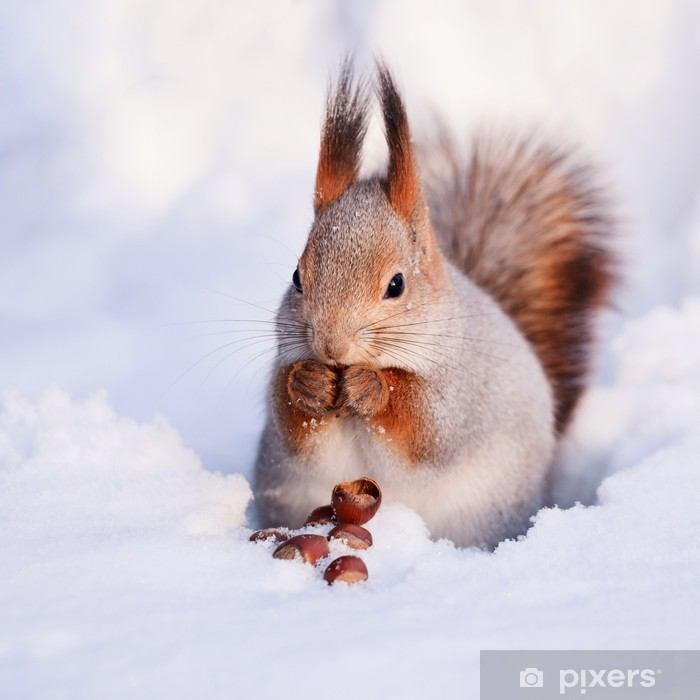
\includegraphics[width=0.6\textwidth]{Testbild.jpg}
	\caption{Ein Eichhörnchen im Schnee}
	\label{fig:eichhoernchen}
\end{figure}
\begin{figure}
	\begin{subfigure}{0.5\textwidth}
		\centering
		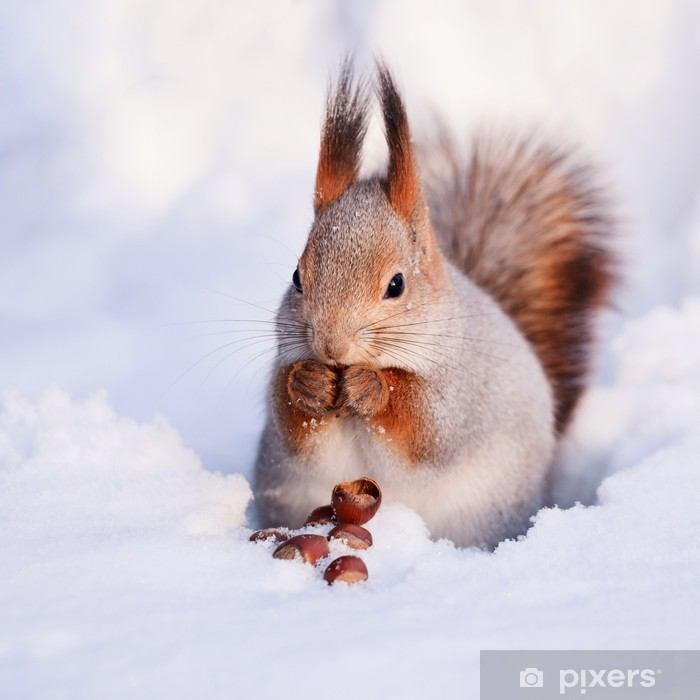
\includegraphics[width=0.95\linewidth]{Testbild.jpg}
		\caption{Eichhörnchen 1}
	\end{subfigure}
	\begin{subfigure}{0.5\textwidth}
		\centering
		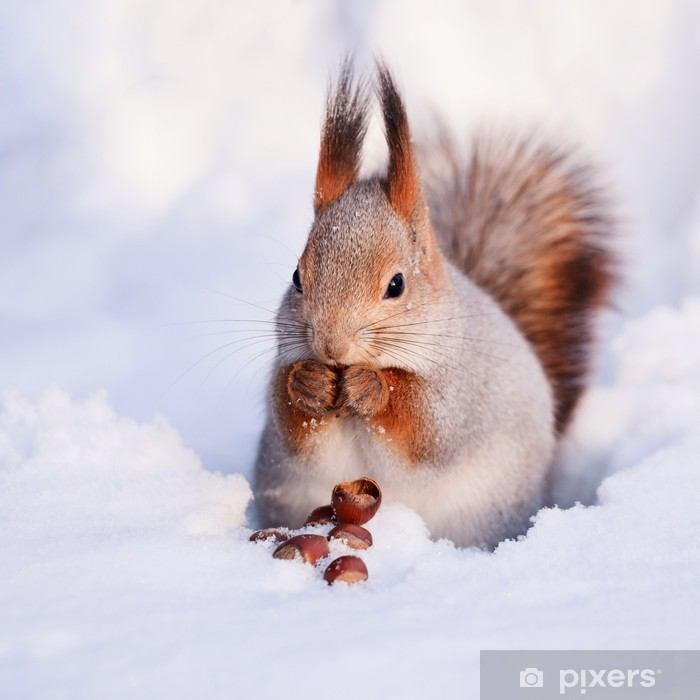
\includegraphics[width=0.95\linewidth]{Testbild.jpg}
		\caption{Eichhörnchen 2}
		\label{subfig:zweitesEichhoernchen}
	\end{subfigure}\\
	\begin{subfigure}{0.5\textwidth}
		\centering
		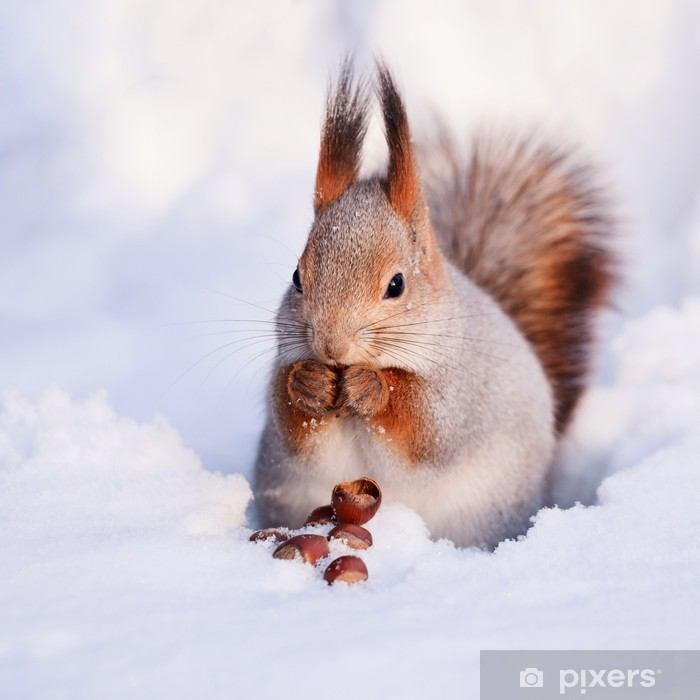
\includegraphics[width=0.95\linewidth]{Testbild.jpg}
		\caption{Eichhörnchen 3}
	\end{subfigure}
	\begin{subfigure}{0.5\textwidth}
		\centering
		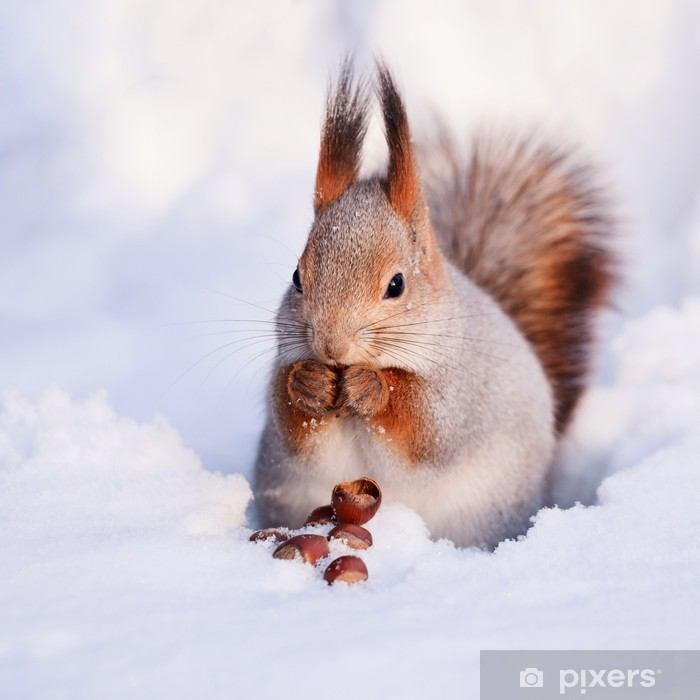
\includegraphics[width=0.95\linewidth]{Testbild.jpg}
		\caption{Eichhörnchen 4}
		\label{subfig:viertesEichhoernchen}
	\end{subfigure}
	\caption{Zwei Eichhörnchen}
\end{figure}
%\subsection und \subsubsection erstellen Unter- und Unterunterkapitel. Diese erscheinen standardmäßig noch im Inhaltsverzeichnis und bekommen eine eigene Überschriftszeile. \paragraph erstellt einen Paragrafen, der NICHT mehr im Inhaltsverzeichnis erscheint und auch keine eigene Überschriftszeile bekommt. Wenn man möchte, dass ein (Unter-/Unterunter-)Kapitel nicht im Inhaltsverzeichnis erscheint (und dementsprechend auch keine Nummer erhält), so schreibt man \section*{...} anstatt \section{} und analog auch für sub- und subsubsection.
\section{Zitieren macht Spaß.}
Wenn wir jetzt den Artikel von Forster 1972 zitieren möchten, dann geben wir \cite{Forster1972} ein.
\nocite{ForsterAna1}
\printbibliography
\section{Tabellen}
\begin{table}[H]
	\centering
	\caption{Eine Tabelle.}
	\begin{tabular}{l||ll}
		\hline
		\textit{Spalte 1} & \textbf{Spalte 2} & {\ul Spalte 3} \\ \hline
		Hallo             & wie gehts         & warum          \\ \hline
		1                 & 2                 & 3              \\ \hline
	\end{tabular}
	\label{tab:MeineErsteTabelle}
\end{table}
\end{document}